\documentclass[a4paper,11pt]{article}

\usepackage{fullpage}
\usepackage[usenames,dvipsnames]{color}
\usepackage{hyperref}
\usepackage{amsmath}
\usepackage{amssymb}
\usepackage{tikz}
\usepackage{tabularx}
\usepackage{booktabs}
\usepackage{amsmath}
\usepackage{multirow}
\usepackage{layouts}
\usepackage{array}
\usepackage{pgf}
\usepackage{tikz}

\usepackage{amssymb}
\usepackage{graphics}
\usepackage{fancyhdr}
\usepackage{eucal}
\usepackage{ifthen}
\usepackage{ifpdf}
\usepackage{lmodern}
\usepackage{amsthm}
\usepackage{catoptions} % For \Autoref

\usetikzlibrary{positioning}

\hypersetup{
  colorlinks,%
    citecolor=black,%
    filecolor=black,%
    linkcolor=black,%
    urlcolor=mygreylink     % can put red here to visualize the links
}

\newcommand{\Pred}[2]{\ensuremath{\mathtt{Predator}\left<#1, #2\right>}}
\newcommand{\Prey}[2]{\ensuremath{\mathtt{Prey}\left<#1, #2\right>}}
\newcommand{\p}[2]{\ensuremath{\mathtt{P}\left<#1, #2\right>}}

\newcommand{\DrawSmallPred}[2]{\node at (A.center #1 #2) {$\pi$};}
\newcommand{\DrawSmallPrey}[2]{\node at (A.center #1 #2) {P};}
\newcommand{\DrawBigPred}[2]  {\node at (A.center #1 #2) {\Huge $\pi$};}
\newcommand{\DrawBigPrey}[2]  {\node at (A.center #1 #2) {\Huge P};}

\definecolor{mygrey}{gray}{.85}
\definecolor{mygreylink}{gray}{.30}
\textheight=8.6in
\raggedbottom
\raggedright

\makeatletter
%% Provide \Autoref; the \autoref with a printed capital
\def\figureautorefname{figure}
\def\tableautorefname{table}
\def\partautorefname{part}
\def\appendixautorefname{appendix}
\def\equationautorefname{equation}
\def\AMSautorefname{equation}
\def\theoremautorefname{theorem}
\def\enumerationautorefname{case}
\def\Autoref#1{%
  \begingroup
  \edef\reserved@a{\cpttrimspaces{#1}}%
  \ifcsndefTF{r@#1}{%
    \xaftercsname{\expandafter\testreftype\@fourthoffive}
      {r@\reserved@a}.\\{#1}%
  }{%
    \ref{#1}%
  }%
  \endgroup
}
\def\testreftype#1.#2\\#3{%
  \ifcsndefTF{#1autorefname}{%
    \def\reserved@a##1##2\@nil{%
      \uppercase{\def\ref@name{##1}}%
      \csn@edef{#1autorefname}{\ref@name##2}%
      \autoref{#3}%
    }%
    \reserved@a#1\@nil
  }{%
    \autoref{#3}%
  }%
}

% For drawing grids
\pgfkeys{/pgf/grid lines/.initial=2}

\pgfdeclareshape{grid}{
    % inherit most things from the rectangle shape
    \inheritsavedanchors[from=rectangle]
    \inheritanchorborder[from=rectangle]
    \inheritanchor[from=rectangle]{center}
    \inheritanchor[from=rectangle]{north}
    \inheritanchor[from=rectangle]{south}
    \inheritanchor[from=rectangle]{west}
    \inheritanchor[from=rectangle]{east}
    \inheritanchor[from=rectangle]{south east}
    \inheritanchor[from=rectangle]{south west}
    \inheritanchor[from=rectangle]{north east}
    \inheritanchor[from=rectangle]{north west}
    \inheritbackgroundpath[from=rectangle]

    \savedmacro\lines{%
        \pgfmathtruncatemacro\lines{\pgfkeysvalueof{/pgf/grid lines}}%
    }

    % draw the grid
    \beforebackgroundpath{
        % store lower right in xa/ya and upper right in xb/yb
        \southwest \pgf@xa=\pgf@x \pgf@ya=\pgf@y
        \northeast \pgf@xb=\pgf@x \pgf@yb=\pgf@y

        % compute distance between the lines
        \pgfmathparse{(\the\pgf@xb-\the\pgf@xa)/(\lines + 1)}
        \pgf@xc=\pgfmathresult pt
        \pgfmathparse{(\the\pgf@yb-\the\pgf@ya)/(\lines + 1)}
        \pgf@yc=\pgfmathresult pt

        % draw grid
        \c@pgf@counta=0
        \c@pgf@countb\lines\relax
        \pgf@xb=\pgf@xa
        \advance\pgf@xb\pgf@xc\relax
        \pgfmathloop
            \ifnum\c@pgf@counta<\c@pgf@countb
                \pgfpathmoveto{\pgfpoint{\pgf@xb}{\pgf@ya}}
                \pgfpathlineto{\pgfpoint{\pgf@xb}{\pgf@yb}}
                \advance\c@pgf@counta 1\relax
                \advance\pgf@xb\pgf@xc\relax
        \repeatpgfmathloop
        % set \pgf@xb to the right side
        \c@pgf@counta=0
        \pgf@yb=\pgf@ya
        \advance\pgf@yb\pgf@yc\relax
        \pgfmathloop
            \ifnum\c@pgf@counta<\c@pgf@countb
                \pgfpathmoveto{\pgfpoint{\pgf@xa}{\pgf@yb}}
                \pgfpathlineto{\pgfpoint{\pgf@xb}{\pgf@yb}}
                \advance\c@pgf@counta 1\relax
                \advance\pgf@yb\pgf@yc\relax
        \repeatpgfmathloop
        \pgfusepath{stroke}
    }

    % add anchors for vertices (intersections of grid lines)
    % and center points (centers of the small rectangles).
    %
    % vertex anchors are simply called 'x y' with '0 0' being the lower left
    % vertex.
    % center anchors are called 'center x y' with 'center 1 1' being the center
    % of the lower left rectangle
    \pgfutil@g@addto@macro\pgf@sh@s@grid{%
        \c@pgf@counta\lines
        \advance\c@pgf@counta 1\relax
        \pgfmathloop\ifnum\c@pgf@counta>-1
            {% group to allow nesting of loops
                \c@pgf@countb\lines
                \advance\c@pgf@countb 1\relax
                \pgfmathloop\ifnum\c@pgf@countb>-1
                    \pgfutil@ifundefined{pgf@anchor@grid@\the\c@pgf@counta\space\the\c@pgf@countb}{%
                        % need to use xdef, so that \c@pgf@counta/b are expanded
                        % vertices
                        \expandafter\xdef\csname pgf@anchor@grid@\the\c@pgf@counta\space\the\c@pgf@countb\endcsname{%
                            \noexpand\southwest \noexpand\pgf@xa=\noexpand\pgf@x \noexpand\pgf@ya=\noexpand\pgf@y
                            \noexpand\northeast \noexpand\pgf@xb=\noexpand\pgf@x \noexpand\pgf@yb=\noexpand\pgf@y
                            \noexpand\pgfmathparse{(\noexpand\the\noexpand\pgf@xb-\noexpand\the\noexpand\pgf@xa)/(\noexpand\lines + 1)*\the\c@pgf@counta}
                            \noexpand\pgf@x=\noexpand\pgf@xa\noexpand\relax
                            \noexpand\advance\noexpand\pgf@x\noexpand\pgfmathresult pt\noexpand\relax
                            \noexpand\pgfmathparse{(\noexpand\the\noexpand\pgf@yb-\noexpand\the\noexpand\pgf@ya)/(\noexpand\lines + 1)*\the\c@pgf@countb}
                            \noexpand\pgf@y=\noexpand\pgf@ya\noexpand\relax
                            \noexpand\advance\noexpand\pgf@y\noexpand\pgfmathresult pt\noexpand\relax
                        }
                        % centers
                        \expandafter\xdef\csname pgf@anchor@grid@center\space\the\c@pgf@counta\space\the\c@pgf@countb\endcsname{%
                            \noexpand\southwest \noexpand\pgf@xa=\noexpand\pgf@x \noexpand\pgf@ya=\noexpand\pgf@y
                            \noexpand\northeast \noexpand\pgf@xb=\noexpand\pgf@x \noexpand\pgf@yb=\noexpand\pgf@y
                            \noexpand\pgfmathparse{(\noexpand\the\noexpand\pgf@xb-\noexpand\the\noexpand\pgf@xa)/(2*(\noexpand\lines + 1))*(2*\the\c@pgf@counta-1)}
                            \noexpand\pgf@x=\noexpand\pgf@xa\noexpand\relax
                            \noexpand\advance\noexpand\pgf@x\noexpand\pgfmathresult pt\noexpand\relax
                            \noexpand\pgfmathparse{(\noexpand\the\noexpand\pgf@yb-\noexpand\the\noexpand\pgf@ya)/(2*(\noexpand\lines + 1))*(2*\the\c@pgf@countb-1)}
                            \noexpand\pgf@y=\noexpand\pgf@ya\noexpand\relax
                            \noexpand\advance\noexpand\pgf@y\noexpand\pgfmathresult pt\noexpand\relax
                        }
                    }{\c@pgf@countb0\relax}
                    \advance\c@pgf@countb-1\relax
                \repeatpgfmathloop
            }
            \advance\c@pgf@counta-1\relax
        \repeatpgfmathloop
    }
}
\makeatother

\tikzset{smallgrid/.style={
            draw,
            grid,
            grid lines=10,
            minimum width=5cm,
            minimum height=5cm}
        }
\tikzset{biggrid/.style={
            draw,
            grid,
            grid lines=10,
            minimum width=15cm,
            minimum height=15cm}
        }
% End of code for grids

\newcommand{\resheading}[1]{{\large \colorbox{mygrey}{\begin{minipage}{\textwidth}{\textbf{#1 \vphantom{p\^{E}}}}\end{minipage}}}}

\newcommand{\mywebheader}{
  \begin{tabular}{@{}p{5in}p{4in}}
  {\resheading{Assignment 1: Single Agent Planning}} & {\Large 21 September, 2012}\\\vspace{0.2cm}
  \end{tabular}}

\begin{document}


\begin{center}
{\LARGE \textbf{Autonomous Agents}}\\ [1em]
\end{center}
\mywebheader

\begin{center}
{\Large By:} \\ \vspace{0.1cm}
{\Large Paris Mavromoustakos} \\  \vspace{0.1cm}
{\Large Georgios Methenitis} \\ \vspace{0.1cm}
{\Large Patrick de Kok} \\ \vspace{0.1cm}
{\Large Marios Tzakris}
\end{center}




\section*{Introduction}
The purpose of this first assignment was to implement a reinforcement learning task that satisfies the Markov property, known as Markov Decision Process (MDP). To achieve this we used one prey, which is part of the environment and behaves in a known probabilistic way, and one agent, the predator, whose goal is to catch the prey. When that happens the episode ends. The environment we used is a 11 by 11 toroidal grid. Also we assumed that the entire MDP is known to our agent. The agent could thus determine the optimal policy even before interacting with the environment. To program the assignment we used the programming language Java.






\section*{Exercise 1}
In the first part, we simulated the environment keeping the policies of the predator and the prey separate. The environment has the ability to hold one or more predators and one or more preys. The predator starts from position $\left<0,0\right>$ and the prey from $\left<5,5\right>$ moving randomly and depending on the given probabilities. Each episode of the simulation ends when the predator catches the prey. Or in case that there are multiple preys and predators the episode ends when there is no alive prey into the simulation environment. In this first assignment we held all of our experiments with one predator and one prey. In Table~\ref{tab:SimStat} we present the overall statistics for this part of the assignment.

\begin{table}[h!]
\caption{Statistics of the simulation over 100 runs.}
\label{tab:SimStat}
\begin{center}
\begin{small}
\begin{tabular}{|@{ }l@{ }|@{ }c@{ }|}
    \hline
     	Average steps & 279.7 \\ \hline
  		Max no. of steps & 1350   \\ \hline
  		Min no. of steps & 22	\\ \hline
  		Mean over 100 runs & 279.7	\\ \hline
  		Stdev over 100 runs & 255.1	\\
    \hline
    \end{tabular}      
\end{small}
\end{center}	
\end{table}





\section*{Exercise 2}
In order to evaluate the random policy we implemented Policy Evaluation, computing the state-value function $V^{\pi_{(S)}}$ and determined the value for each state. For all $s \in S$,
\[
V^{\pi_{(S)}} = \sum_{a}\pi(s,a)\sum_{s'}P_{ss'}^a[R_{ss'}^a + \gamma V^{\pi}(s')]
\]
First, in the naive approach we computed the state value function for every state in the $11^{4}$ space. The produced values for the given states are presented:

\begin{align*}
	V^{\pi_{(S)}}(\left\{\Pred{0}{0},\Prey{5}{5}\right\})   & = 0.0008 \\
    V^{\pi_{(S)}}(\left\{\Pred{2}{3},\Prey{5}{4}\right\})   &= 0.8900 \\
    V^{\pi_{(S)}}(\left\{\Pred{2}{10},\Prey{10}{0}\right\}) &= 0.8900 \\
    V^{\pi_{(S)}}(\left\{\Pred{10}{10},\Prey{0}{0}\right\}) &= 0.8817
\end{align*}

Except from the naive state space we accomplished to reduce the state space in $6^2$, and finally in 21. Trying to implement the Policy Evaluation algorithm on the reduced state space, we acquire the same values as above, however, we noticed that the algorithm runs significantly faster. Table presents the performance results we had performing this algorithm to smaller state spaces than the original one. We set $\theta$ variable to zero in order our algorithm to produce more accurate results. This may cause an increase in our algorithm's execution time.

\begin{table}[h!]
\caption{Policy Evaluation algorithm performance.}
\label{peap}
\begin{center}
\begin{tabular}{c@{ }@{ }c@{ }@{ }c@{ }@{ }c}
\textbf{State Space} & \textbf{D. Factor} & \textbf{Iterations} & \textbf{Time of Execution (ms.)} \\
\midrule
$11^{4}$ 		& 0.9 				& 202 				& 245608 \\
				& 0.7 				& 73 				& 94660 	 \\
 				& 0.5 				& 46 				& 57754 	 \\
 				& 0.1 				& 23 				& 29467 \vspace{0.1cm} \\ 
$6^{2}$			& 0.9 				& 215 				& 821 	 \\ 
				& 0.7 				& 72 				& 369  \\
				& 0.5 				& 44 				& 283 	 \\
				& 0.1 				& 16 				& 114 	\vspace{0.1cm}  \\ 
$21$ 			& 0.9 				& 215 				& 475  \\ 
	 			& 0.7 				& 72 				& 280  \\
	 			& 0.5 				& 41 				& 195  \\
	 			& 0.1 				& 16 				& 50  \\
\end{tabular}
\end{center}
\end{table}



\newpage
\section*{Exercise 3}
When naively exploring the state space $\mathcal{S}$, you will have to compute the value for all possible states, depending on four variables (the coordinates of both the predator and prey), each of which can have 11 different values.  This results in $11^4 = 14641$ different states.  Because of the toroidal structure of the world, the state $\left\{\Pred{x}{y}, \Prey{x'}{y'}\right\}$ is equivalent to $\left\{\Pred{x+a}{y+b}, \Prey{x'+a}{y'+b}\right\}$; there is no special square in the given world which has features that distinguish it from other squares.  From this follows that we can fix either $x, y$ or $x', y'$ to a certain value.  By doing so, we have removed two degrees of freedom, and reduced the space to only $11^2 = 121$ unique states.  Note that, when the position of the predator and prey are seen as vectors, this represents the difference vector $\Pred{x}{y} - \Prey{x'}{y'}$ or $\Prey{x'}{y'} - \Pred{x}{y}$, when respectively $x', y'$ or $x, y$ are fixed.  We have chosen to fix $x', y'$, and with $\p{x}{y}$ we denote the class of states for which $\left\{\Pred{x+a}{y+b}, \Prey{a}{b}\right\}$ holds.
\begin{figure}
\begin{center}
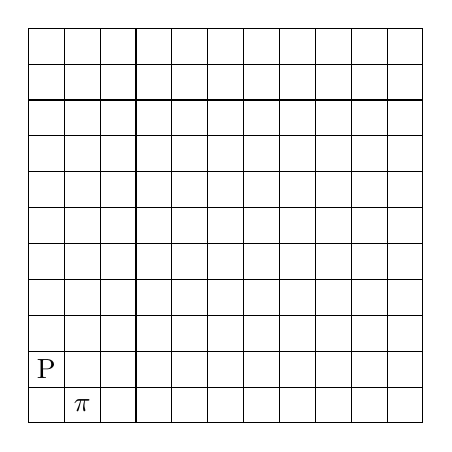
\begin{tikzpicture}
\node [smallgrid] (A) at (0,0) {};
\DrawSmallPrey{1}{2} 
\DrawSmallPred{2}{1}
\end{tikzpicture}
\end{center}
\end{figure}

\section*{Exercise 4}
To find an optimal policy we computed the optimal value function $V^\ast$ for all states. First of all, we had to find the value function for the naive $11^4$ state space. For all $s \in S$,
\[
V^{\pi_{(S)}} = \max_{a} \sum_{s'}P_{ss'}^a[R_{ss'}^a + \gamma V^{\pi}(s')]
\]
Table~\ref{viat} presents the value table that was computed with the value iteration algorithm for a discount factor $\gamma = 0.7$ and $\theta = 0$. 
\begin{table}[h!]
\caption{Value Iteration algorithm performance, $\pi = \langle 5,5 \rangle$, $\gamma = 0.7$, $\theta = 0$.}
\label{viat}
\begin{center}
\begin{tabular}{|c|c|c|c|c|c|c|c|c|c|c|}
\hline
0.44 & 0.61 & 0.85 & 1.18 & 1.65 & 2.13 & 1.65 & 1.18 & 0.85 & 0.61 & 0.44 \\ \hline
0.61 & 0.84 & 1.18 & 1.67 & 2.35 & 3.09 & 2.35 & 1.67 & 1.18 & 0.84 & 0.61 \\ \hline
0.85 & 1.18 & 1.67 & 2.35 & 3.32 & 4.50 & 3.32 & 2.35 & 1.67 & 1.18 & 0.85 \\ \hline
1.18 & 1.67 & 2.35 & 3.32 & 4.69 & 6.55 & 4.69 & 3.32 & 2.35 & 1.67 & 1.18 \\ \hline
1.65 & 2.35 & 3.32 & 4.69 & 6.55 & 10.00 & 6.55 & 4.69 & 3.32 & 2.35 & 1.65 \\ \hline
2.13 & 3.09 & 4.50 & 6.55 & 10.00 & $\pi$ & 10.00 & 6.55 & 4.50 & 3.09 & 2.13 \\ \hline
1.65 & 2.35 & 3.32 & 4.69 & 6.55 & 10.00 & 6.55 & 4.69 & 3.32 & 2.35 & 1.65 \\ \hline
1.18 & 1.67 & 2.35 & 3.32 & 4.69 & 6.55 & 4.69 & 3.32 & 2.35 & 1.67 & 1.18 \\ \hline
0.85 & 1.18 & 1.67 & 2.35 & 3.32 & 4.50 & 3.32 & 2.35 & 1.67 & 1.18 & 0.85 \\ \hline
0.61 & 0.84 & 1.18 & 1.67 & 2.35 & 3.09 & 2.35 & 1.67 & 1.18 & 0.84 & 0.61 \\ \hline
0.44 & 0.61 & 0.85 & 1.18 & 1.65 & 2.13 & 1.65 & 1.18 & 0.85 & 0.61 & 0.44 \\ \hline
\end{tabular}
\end{center}
\end{table}
We also implemented the Value Iteration algorithm on the reduced state space, acquiring the same values as above, however, we noticed that the algorithm runs significantly faster. Table presents the performance results we had performing this algorithm to smaller state spaces than the original one. We set $\theta$ variable to zero in order our algorithm to produce more accurate results. This may cause an increase in the execution time of the Value Iteration algorithm.


\begin{table}[h!]
\caption{Value Iteration algorithm results. }
\label{viap}
\begin{center}
\begin{tabular}{c@{ }@{ }c@{ }@{ }c@{ }@{ }c}
\textbf{State Space} & \textbf{D. Factor} & \textbf{Iterations} & \textbf{Time of Execution (ms.)} \\
\midrule
$11^{4}$ 		& 0.9 				& 29 				& 37774 \\
				& 0.7 				& 26 				& 34423 	 \\
 				& 0.5 				& 24 				& 31848 	 \\
 				& 0.1 				& 19 				& 24883  \vspace{0.1cm}  \\ 
$6^{2}$			& 0.9 				& 22 				& 229 	 \\
				& 0.7 				& 19 				& 162  \\
				& 0.5 				& 16 				& 126 	 \\
				& 0.1 				& 11 				& 88 	 \vspace{0.1cm}  \\ 
$21$ 			& 0.9 				& 22 				& 93  \\
	 			& 0.7 				& 19 				& 70  \\
	 			& 0.5 				& 17 				& 67  \\
	 			& 0.1 				& 11 				& 60  \\
\end{tabular}
\end{center}
\end{table}

\section*{Exercise 5}
To iteratively improve the policy we implemented policy iteration $V^{\pi^\prime}$ for all states which the prey is located at $\left<5,5\right>$.

The convergence speed (in number of iterations) for different discount factors $\gamma$ is presented in \autoref{tab:convPI}.
\begin{table}
\caption{Trololol.}
\label{tab:convPI}
\begin{center}
\begin{tabular}{|@{ }r@{ }|@{ }r@{ }|}
\hline
Discount factor $\gamma$ & Number of iterations \\
\hline
0.1 & \\
0.5 & \\
0.7 & \\
0.9 & \\
\hline
\end{tabular}
\end{center}
\end{table}

\end{document}